%%%%%%%%%%%%%%%%%%%%%%%%%%%%%%%%%%%%%%%%%
% written by: Ruben (rg@ht11.org)
%%%%%%%%%%%%%%%%%%%%%%%%%%%%%%%%%%%%%%%%%

\documentclass{article}
\usepackage{fancyhdr} % Nice headers
\usepackage{lastpage} % Required to determine the last page for the footer
\usepackage{extramarks} % Required for headers and footers
\usepackage{graphicx} % Required to insert images
\usepackage{listings} % Required for insertion of code
\usepackage{courier} % Required for the courier font
\usepackage[hidelinks]{hyperref} % I hate hyperlinks in docs...
\usepackage[utf8]{inputenc} % because äöü
\usepackage{setspace} % Spacing between rows

% Margins
\topmargin=-0.45in
\evensidemargin=0in
\oddsidemargin=0in
\textwidth=6.5in
\textheight=9.0in
\headsep=0.25in

\linespread{1.1} % Line spacing

% Set up the header and footer
\pagestyle{fancy}
% \lhead{Ruben Gonzalez} % Top left header
\chead{Computer Networks Cheat Sheet} % Top center head
\rhead{} % Top right header
\lfoot{\copyright Ruben, released under the BEERWARE license} % Bottom left footer
\cfoot{} % Bottom center footer
\rfoot{Page\ \thepage\ of \pageref*{LastPage}} % Bottom right footer, * so hyperref doesnt link it.
\renewcommand\headrulewidth{0.4pt} % Size of the header rule
\renewcommand\footrulewidth{0.4pt} % Size of the footer rule

\setlength\parindent{0pt} % Removes all indentation from paragraphs

\begin{document}
\section{Packet Delay}
\subsection{Definitions}
\textbf{Link capacity}
Capacity of link. Unit: $\frac{Bits}{Seconds}$.

\textbf{Transmission Delay}
Time needed to bring bytes of packet onto link. Calculated: $d_{trans} = \frac{B}{R}$, with B = bits per packet and R = Link Capacity.

\textbf{Propragation Delay}
Time neeeded to transmit one bit from one end of the link to the other. 

\textbf{Processing Delay}
Time needed to proccess packet.

\textbf{Queueing Delay}
Time spend waiting in buffer queues.

\textbf{Overall Delay}
Calculated: $d_{nodal} = d_{proc} + d_{queue} + d_{trans} + d_{prop}$

\begin{flushleft}
	\textbf{End to End Delay} [\textit{Übertragungsdauer}]\linebreak
	Also Known as one way delay. Time needed for packet to go from sender to receipient. Usually $\frac{RTT}{2}$. Excact: $T_{e2e} = \sum\limits_{i}^{n} d_{i}$, with $d_{i}$ = overall delay of network segment i. 
\end{flushleft}


\textbf{End to End Delay for Multiple Packages}
$T_{e2e}(n) = T_{e2e}(1) + (n-1) \cdot \frac{L}{B}$, with L = Size of one packet, B = Bandwidth of Bottleneck, n = number of Packages.

\section{HTTP}
\subsection{Definitions}
\textbf{Non Persistent HTTP}
One HTTP request per TCP connection.

\textbf{Persistent HTTP}
Multiple HTTP request per TCP connection. Still one request at a time, next HTTP request gets send after previous HTTP request is done.

\textbf{Pipelining HTTP}
Introduced in HTTP/1.1. Send multiple ordered requests simultaniously, without waiting for previous requests to be done.

\begin{figure}[h]
    \centering
    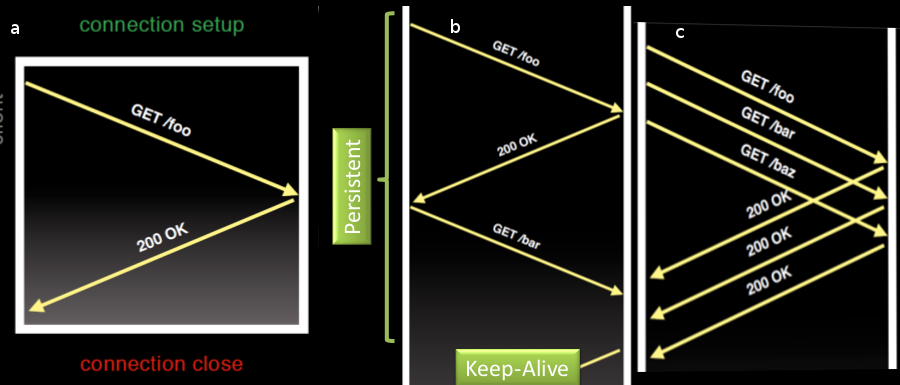
\includegraphics[width=0.9\textwidth]{media/http.png}
    \caption{Different HTTP versions. a non persistent, b persistent, c pipelined HTTP}
    \label{fig:pipe_http}
\end{figure}

\pagebreak

\section{TCP Flow Control}
\subsection{Definitions}
\label{sbsec:flow_defs}
\textbf{Window}
Bytes allowed to be sent before receiving next ACK.


\textbf{Window Size}
Size of window. Basically size of receipient buffer.

\textbf{Advertised Window}
Receipients Window Size told to sender of TCP packets. Maximum size allowed for window.

\textbf{Maximum Segment Size (MSS)}
Payload size in bytes. Usually MTU - len(IP header) - len(TCP header), on ethernet MSS=1460.

\textbf{Window}
Bytes allowed to be sent before receiving next ACK.

\textbf{Segment}
TCP packet. Consists of header and data.

\textbf{Flight Size}
Number of TCP packets send but without ACK received yet.

\textbf{Go-Back-N}
In case a timeout occures, all packages sent after lost packages get resend immediately. 

\textbf{Selective Repeat}
Every packages gets an own ACK. In case timeout occures, only lost package gets resend.

\textbf{Sequence Number (SEQ)[header field]}
Numbering of data within segment. SEQ = first byte in the payload (data) of segment. Gets initialized to random number (ISN) at start of connection.

\textbf{Acknowledge Number (ACK)[header field]}
Acknowledgement of received segments. Value is SEQ + 1, with SEQ = segment number of received segment.

\textbf{Bandwidth-Delay-Product} 
Necessary window size to use the full link capacity.\\
Window in bit: $RTT \cdot C$ \\
Window in packet count: $\frac{RTT \cdot C}{L}$ \\
C is the link capacity, in case there are multiple links the bottleneck link capacity.


\subsection{Sliding Window}
Every time a ACK returns, the sender slides the Window over the bytes to send.
\begin{figure}[h]
    \centering
    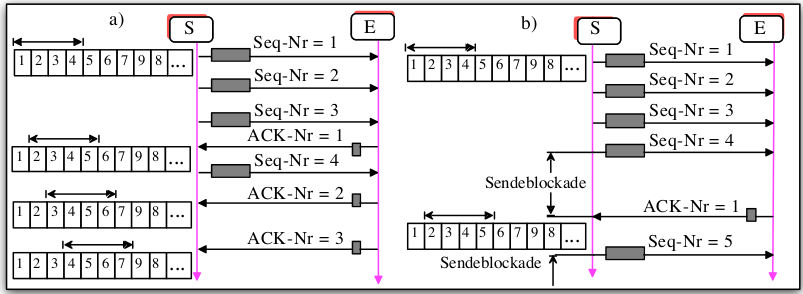
\includegraphics[width=0.6\textwidth]{media/sliding_window.png}
    \caption{Sliding window with Window Size = 4, a without, b with error}
    \label{fig:sliding}
\end{figure}


\section{TCP Efficency Tuning}
\subsection{Definitions}

\textbf{Congestion Window (cwnd)}
The same as Window, see \ref{sbsec:flow_defs}.

\textbf{Slow Start Threshhold (ssthresh)}
Limit until exponential growth (Slow Start) of cwnd is performed. After $cwnd \geq sstresh$, linear growth (congestion avoidance) is performed.

\textbf{Double ACK (dACK)}
In case a segment is missing, the ACK for the already arrived segment with bigger SEQ is repeadiately sent.

\textbf{Packet loss}
Paket is considered lost if either the timeout for ACK is reached, or 3 dACKs have arrived.

\subsection{Slow Start}
Algorithm to perform exponential growth of cwnd.

Begins with $cwnd = 1 \cdot MSS$ and performs $cwnd = cwnd + MSS$ on every received ACK.

\subsection{Congestion Avoidance}
Algorithm to perform linear growth of cwnd if needed.

In case $cwnd \geq sstresh$ occures, cwnd gets increased $cwnd = cwnd + \frac{MSS^{2}}{cwnd}$ everytime a ACK arrives. Otherwise Slow Start is performed.

Congestion avoidance begins with these steps:

\begin{enumerate}
     \item Set $ssthresh = 2^{16} -1 = 65535$
     \item Begin with slow start.
\end{enumerate}

In case a packet loss gets detected, the following is done:

\begin{itemize}
     \item In case a timeout occured: set $ssthresh = max(2, \frac{cwnd}{2})$ and do slow start
     \item In case 3 dACKs were received: only set $ssthresh = max(2, \frac{cwnd}{2})$ (as in 1.)
\end{itemize}

\subsection{Fast Retransmit}
Mechanism that means: On third dACK received, the missing segment gets resent immediately without waiting for timer to expire.

\subsection{Fast Recovery}
Mechanism that means: After fast retransmit, congestion avoidance is performed not slow start.

The usual implementation looks like this: If third dACK is received do the following:

\begin{enumerate}
     \item Set $ssthresh = max(2, \frac{cwnd}{2})$
     \item Retransmit the missing segment
     \item Set $cwnd = ssthresh + 3 \cdot MSS$
     \item Every time another dACK arrives set $cwnd = cwnd + MSS$
     \item Once a ACK for new data arrives, set $cwnd = sstresh$.
\end{enumerate}

\section{Throughput}
\subsection{Definitions}

\textbf{Round Trip Time (RTT)}
Estimation of time needed from sending a package until receving an answer (after leaving link to the answer arriving).

\subsection{Bandwitdh Delay Product}
Measures the throughput: $bdp [\frac{byte}{sec}] = \frac{Windowsize [byte]}{RTT [sec]}$

\section{IP}
\subsection{Whats new}
The usual stuff. Use the most specific (smallest) subnet matching in routing.

\section{Routing Protocols}
\subsection{Routing Information Protocol (RIP)}
Metric is the amount of Hops.

\subsection{Open Shortest Path First (OSPF)}
Metric for route: $\sum{max (\frac{100 Mbits}{Bandwidth}, 1)}$ of all links. So the least possible metric for one single link is 1.

\subsection{Enhanced Gateway Routing Protocol (EGRP)}
Metric for route: $ \frac{10 Gbps}{min(Bandwidth)} + \sum\limits_{link i}^{n} \frac{D_i}{10\mu s}$, with D=Delay

\subsection{Dijkstra}
Algorithm to find shortest path to all nodes.

\begin{figure}[h]
    \centering
    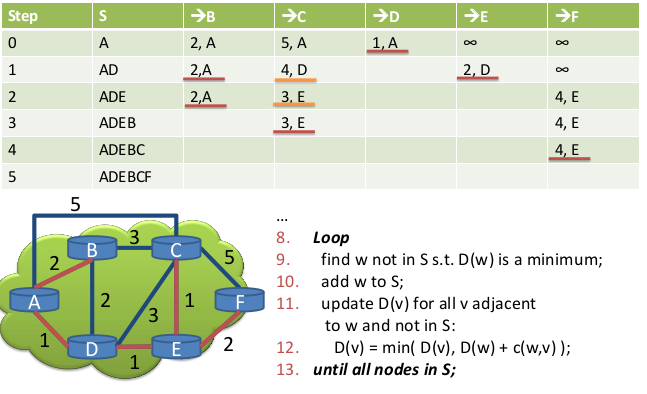
\includegraphics[width=0.6\textwidth]{media/dijkstra.png}
    \caption{Example of the dijkstra algorithm}
    \label{fig:dijkstra}
\end{figure}

\section{Unit-Conversion}
\begin{minipage}{0.49\linewidth}
	\begin{tabular}{|l|r|l|}
		\hline
		\textbf{SI-Unit} & \multicolumn{1}{l|}{\textbf{non SI-Unit}} & \textbf{Factor} \\ \hline
		1s               & 1.000.000.000 ns                          & $ 10^{9} $      \\ \hline
		1s               & 1.000.000 $ \mu $s                                  & $ 10^{6} $      \\ \hline
		1s               & 1.000 ms                                  & $ 10^{3} $      \\ \hline
	\end{tabular}
\end{minipage}
\begin{minipage}{0.49\linewidth}
	\begin{tabular}{|l|r|l|}
		\hline
		\textbf{Unit} & \multicolumn{1}{l|}{\textbf{bytes}} & \textbf{Factor} \\ \hline
		kilo               & 1.000 B                         & $ 10^{3} $      \\ \hline
		mega               & 1.000.000 B                     & $ 10^{6} $      \\ \hline
		giga               & 1.000.000.000 B                 & $ 10^{9} $      \\ \hline
	\end{tabular}
\end{minipage}

\subsection{Decimal - Binary}

\begin{table}[!h]
	\centering
	\begin{tabular}{|l|r|l|l|}
		\hline
		128 & \multicolumn{1}{l|}{1000 0000} & 248 & 1111 1000 \\ \hline
		192 & 1100 0000                      & 252 & 1111 1100 \\ \hline
		224 & 1110 0000                      & 254 & 1111 1110 \\ \hline
		240 & 1111 0000                      & 255 & 1111 1111 \\ \hline
	\end{tabular}
\end{table}

\newpage
\section{Theoriefragen}
\begin{enumerate}
	\item \textbf{Was ist der Unterschied zwischen switching und routing?}
	\begin{flushleft}
		Routing auf IP-Ebene und kann verschiedene Subnetze verwalten, Switching auf MAC-Ebene (haben keine eigene IP).
	\end{flushleft}
	\item \textbf{Wie kann in einem Netz eine Änderung der verschiedenen Knoten/der Links zwischen den Knoten erkannt werden?}
	\begin{itemize}
		\item Broadcast von Hello-Paketen alle 10s, dadurch Erkennung von defekten Nachbarn (default Timeout: 40s)
		\item Broadcast des Link-States bei Veränderung
	\end{itemize}
	\item \textbf{Was sind die Vor- und Nachteile von TCP}
	\begin{itemize}
		\item Vorteile
			\begin{itemize}
				\item Ist Ausfall sicherer als UDP (Verlorene Pakete werden nachgesendet).
			\end{itemize}
		\item Nachteile
			\begin{itemize}
				\item langsamer als UDP 
				\item mehr Nachrichten
			\end{itemize}
	\end{itemize}
	\item \textbf{Was sind die Vor- und Nachteile von UDP}
	\begin{itemize}
		\item Vorteile
		\begin{itemize}
			\item schneller als TCP
			\item weniger Nachrichten
			\item Broadcast möglich
		\end{itemize}
		\item Nachteile
		\begin{itemize}
			\item Verlorene Pakete werden nicht Nachgesendet
		\end{itemize}
	\end{itemize}
	\item \textbf{Wie bestimmt der Browser welche IP-Adresse der zugehörige Webserver hat, und auf welchem Port er Anfragen zum Webserver schicken soll?}
	\begin{itemize}
		\item Anfrage an DNS-Server $ \longrightarrow $ Auflösen der URL in IP (fragt ggf. den nächst höheren)
		\item Port ist Protokollabhängig: http = 80; https = 443
	\end{itemize}
	\item \textbf{Welche Protokolle auf Applikations- und Transportschicht werden verwendet, um Daten zwischen Browser und Webserver zu übertragen?}
	\begin{itemize}
		\item TCP
		\item HTTP(s)
	\end{itemize}
	\item \textbf{Wie funktioniert ein Caching Proxy?}
	\begin{itemize}
		\item \textbf{Aufgabe Proxy}: Entscheiden was aus dem Internet im Cache gespeichert wird und ob angeforderte Daten aus dem Cache geladen werden (können).
		\item \textbf{Aufgabe Cache}: Speichern, Verwalten und Bereitstellen von Daten die er vom Proxy zugeteilt bekommt.
		\item \textbf{Sicherstellung das Cache aktuelle Seite bereitstellt}: Über Timeout von verschiedenen daten
	\end{itemize}

	\item \textbf{Was passiert im Falle von persistent HTTP, wenn der Cache den HTML-Code nicht gespeichert hat? Erklären Sie das Szenario. Eine exakte Berechnung der Page Load Time ist nicht notwendig!}
	\begin{flushleft}
		Zuerst wird der Proxy angefragt, ob die Seite im Cache vorhanden ist. Da dies nicht der Fall ist, wird eine Verbindung aufgebaut, der HTML-Code geholt und anschließend in der selben Verbindung die Bilder.\linebreak
		\textbf{Anmerkung}: Bilder sind im Cache, da aber persistent Verbindung werden alle Bilder trotzdem von Internet geladen, da der Proxy nicht erneut angefragt wird.
	\end{flushleft}
	\item \textbf{Was passiert, wenn der Server persistent http unterstützt, der Cache aber nur non-persistent http? Betrachten Sie den Fall, dass der Cache den HTML-Code und die Hälfte der referenzierten Bilder gespeichert hat. Erklären Sie das Szenario. Eine exakte Berechnung der Page Load Time ist nicht notwendig!}
	\begin{flushleft}
		Dieses mal wird ebenfalls wieder der Proxy angefragt. Alle Elemente, welche im Cache liegen werden per Non-Persistent (jedes Objekt eigene Verbindung) geladen. Die fehlenden Dateien werden über eine Persistent Verbindung aus dem Internet geladen. Wird allerdings ein Element welches nicht im Cache vorhanden ist angefordert, wird eine persistente Verbindung erstellt. Alle weiteren Objekte werden dann über diese Verbindung geladen.\linebreak
		\textbf{Beispiel}: Bild 1,2,4 sind im Cache. Wird jetzt Bild 3 angefordert wird Bild 4 nicht aus dem Cache geladen, sonder über die Persistente Verbindung geladen.
	\end{flushleft}
	
	\item \textbf{Für was wird DNS benötigt und wie ist das Weltweite DNS aufgebaut?}
	\begin{flushleft}
		Wird benötigt um Namen(Domainadressen) in IPs aufzulösen. Der Aufbau von DNS ist hierarchisch angeordnet und die Namensauflösung kann iterativ oder rekursiv gelöst sein.
	\end{flushleft}
	
	\item \textbf{Beschreiben sie in Pseudo-Code die Funktionsweise eines DNS Server.}
	\begin{itemize}
		\item UDP
		\begin{lstlisting}[language=Python]
udpSocket.listen(53)
while True:
	adress, data = udpSocket.blockingReceive()
	udpSocket.send(adress, dnsMap.get(data))
		\end{lstlisting}
	\item TCP
		\begin{lstlisting}[language=Python]
while True:
	socket = waitForTCPConnection()
	new WorkerThread(socket)
	
WorkerTread(tcpSocket):
	data = tcpSocket.blockingreceive()
	tcpSocket.send(dnsMap.get(data))
	tcpSocket.close()
		\end{lstlisting}
	\end{itemize}
	
	\item \textbf{Auf welcher Basis können Pakete dem UDP bzw. TCP Socket auf Port 53 zugewiesen werden?}
	\begin{flushleft}
		IP-Header hat ein Feld welches das Transportprotokoll angibt.
	\end{flushleft}
	
\end{enumerate}

\section{OSI Modell}
\begin{figure}[!ht]
	\centering
	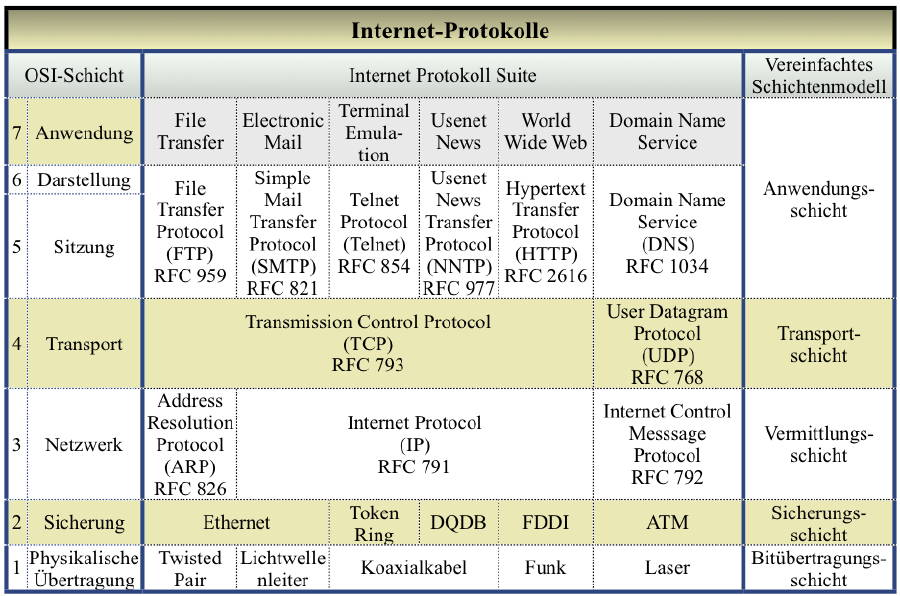
\includegraphics[scale=0.5]{media/OSI-Modell}
\end{figure}

\end{document}

